% Preamble: Setting up the document with required packages
\documentclass[12pt]{standalone}
\usepackage{tikz}
\usetikzlibrary{shapes.geometric, arrows.meta, positioning, calc}
\usepackage{amsmath, amssymb} % For mathematical symbols if needed
\usepackage{times} % Use Times font, compatible with PDFLaTeX

% Begin document
\begin{document}

% Adding vertical space to move the chart down by approximately 1 inch (2.54 cm)
\vspace{2.54cm} % <--- Added to shift the entire chart down by 1 inch

% Creating the hierarchy chart using TikZ
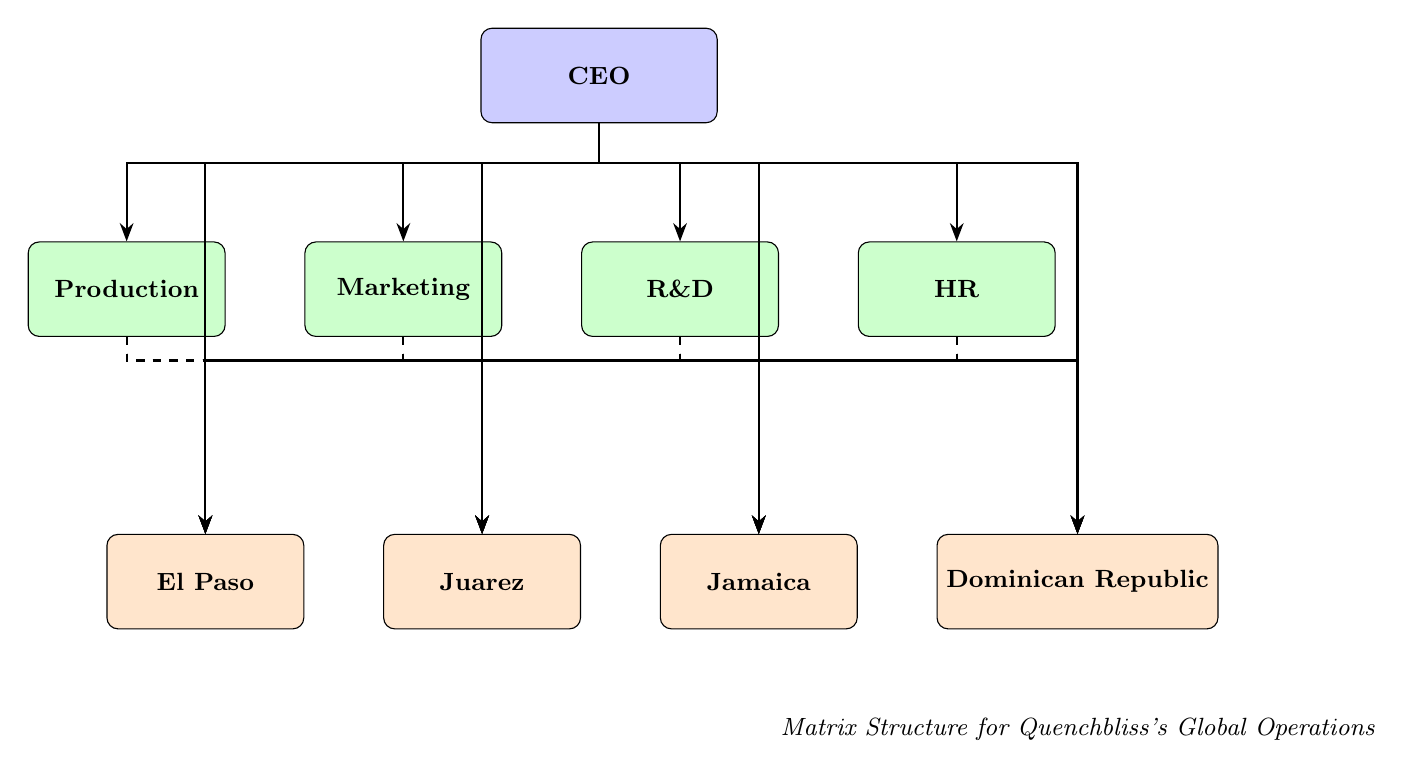
\begin{tikzpicture}[
    % Define node styles
    box/.style={rectangle, draw, rounded corners, minimum height=1.2cm, minimum width=2.5cm, align=center, font=\small\bfseries},
    ceo/.style={box, fill=blue!20, minimum width=3cm},
    func/.style={box, fill=green!20},
    geo/.style={box, fill=orange!20},
    % Define edge style
    edge/.style={-Stealth, thick},
    % Spacing adjustments
    level distance=2cm,
    sibling distance=2.5cm,
]

% Drawing the CEO node at the top
\node[ceo] (CEO) {CEO};

% Drawing the Functional divisions row
\node[func, below=1.5cm of CEO, xshift=-6cm] (Production) {Production};
\node[func, right=1cm of Production] (Marketing) {Marketing};
\node[func, right=1cm of Marketing] (RD) {R\&D};
\node[func, right=1cm of RD] (HR) {HR};

% Drawing the Geographic divisions row
\node[geo, below=2.5cm of Production, xshift=1cm] (ElPaso) {El Paso};
\node[geo, right=1cm of ElPaso] (Juarez) {Juarez};
\node[geo, right=1cm of Juarez] (Jamaica) {Jamaica};
\node[geo, right=1cm of Jamaica] (Dominican) {Dominican Republic};

% Connecting the CEO to Functional divisions
\foreach \func in {Production, Marketing, RD, HR} {
    \draw[edge] (CEO.south) -- ++(0,-0.5) -| (\func.north);
}

% Connecting the CEO to Geographic divisions
\foreach \geo in {ElPaso, Juarez, Jamaica, Dominican} {
    \draw[edge] (CEO.south) -- ++(0,-0.5) -| (\geo.north);
}

% Adding dashed lines to show dual reporting (matrix structure) between Functional and Geographic divisions
\foreach \func in {Production, Marketing, RD, HR} {
    \foreach \geo in {ElPaso, Juarez, Jamaica, Dominican} {
        \draw[dashed, edge] (\func.south) -- ++(0,-0.3) -| (\geo.north);
    }
}

% Adding a caption below the chart
\node[below=1cm of Dominican, font=\small\itshape] {Matrix Structure for Quenchbliss's Global Operations};

\end{tikzpicture}

\end{document}